\documentclass[a4paper]{scrartcl}
\usepackage{mystyle1}
\usepackage{bm}
\usepackage{tikz}
\usepackage{dashrule}
\usepackage{array}
\usepackage{microtype}
\usepackage{mathtools}
\usepackage[left=2cm, right=2cm, top=2cm, bottom=2cm]{geometry}
%\usepackage{adjustbox}
%\usepackage{mathrsfs}
%\usepackage{cancel}
\usepackage{hyperref}
\hypersetup{
        colorlinks=true,
        urlcolor=RubineRed,
        linkcolor=RoyalBlue!90!black,
        citecolor=retrocyan,
        breaklinks=true
    }



\addtokomafont{title}{\sffamily}
\setkomafont{subtitle}{\LARGE\sffamily\bfseries}
\DeclareFontShape{T1}{cmss}{b}{n}{<->ssub*cmss/bx/n}{}
\setkomafont{author}{\large}
\setkomafont{date}{}


\title{
        \Large\textsc{CS3101 Project: Flight Reservation System} \\
        \vspace{10pt}
        \Huge\textbf{Ronway Airlines} \\
}


\author{Ronit Bhuyan \\ \texttt{22MS025} \and Sagnik Seth \\ \texttt{22MS026} \and   Aviyank Aryan \\ \texttt{22MS030}}
\date{}




\begin{document}
\maketitle
\tableofcontents
\section{Introduction}
This project is made as part of the CS3101 course. The project is a flight reservation system which is named as Ronway Airlines. The project is made using C and compiled using gcc. The system can be accessed in two modes: User and Admin. As a User, one can search flights according to the source,destination, date and time. The user can also book a flight, cancel a booking, view the booking history and also chat with the chatbot named Bandhu. As an Admin, one can add flights, view all the flights available, change the details of a flight and delete a flight altogether.
\section{Building and Dependencies}
\section{Main Structure}


\begin{figure}[H]
    \centering
    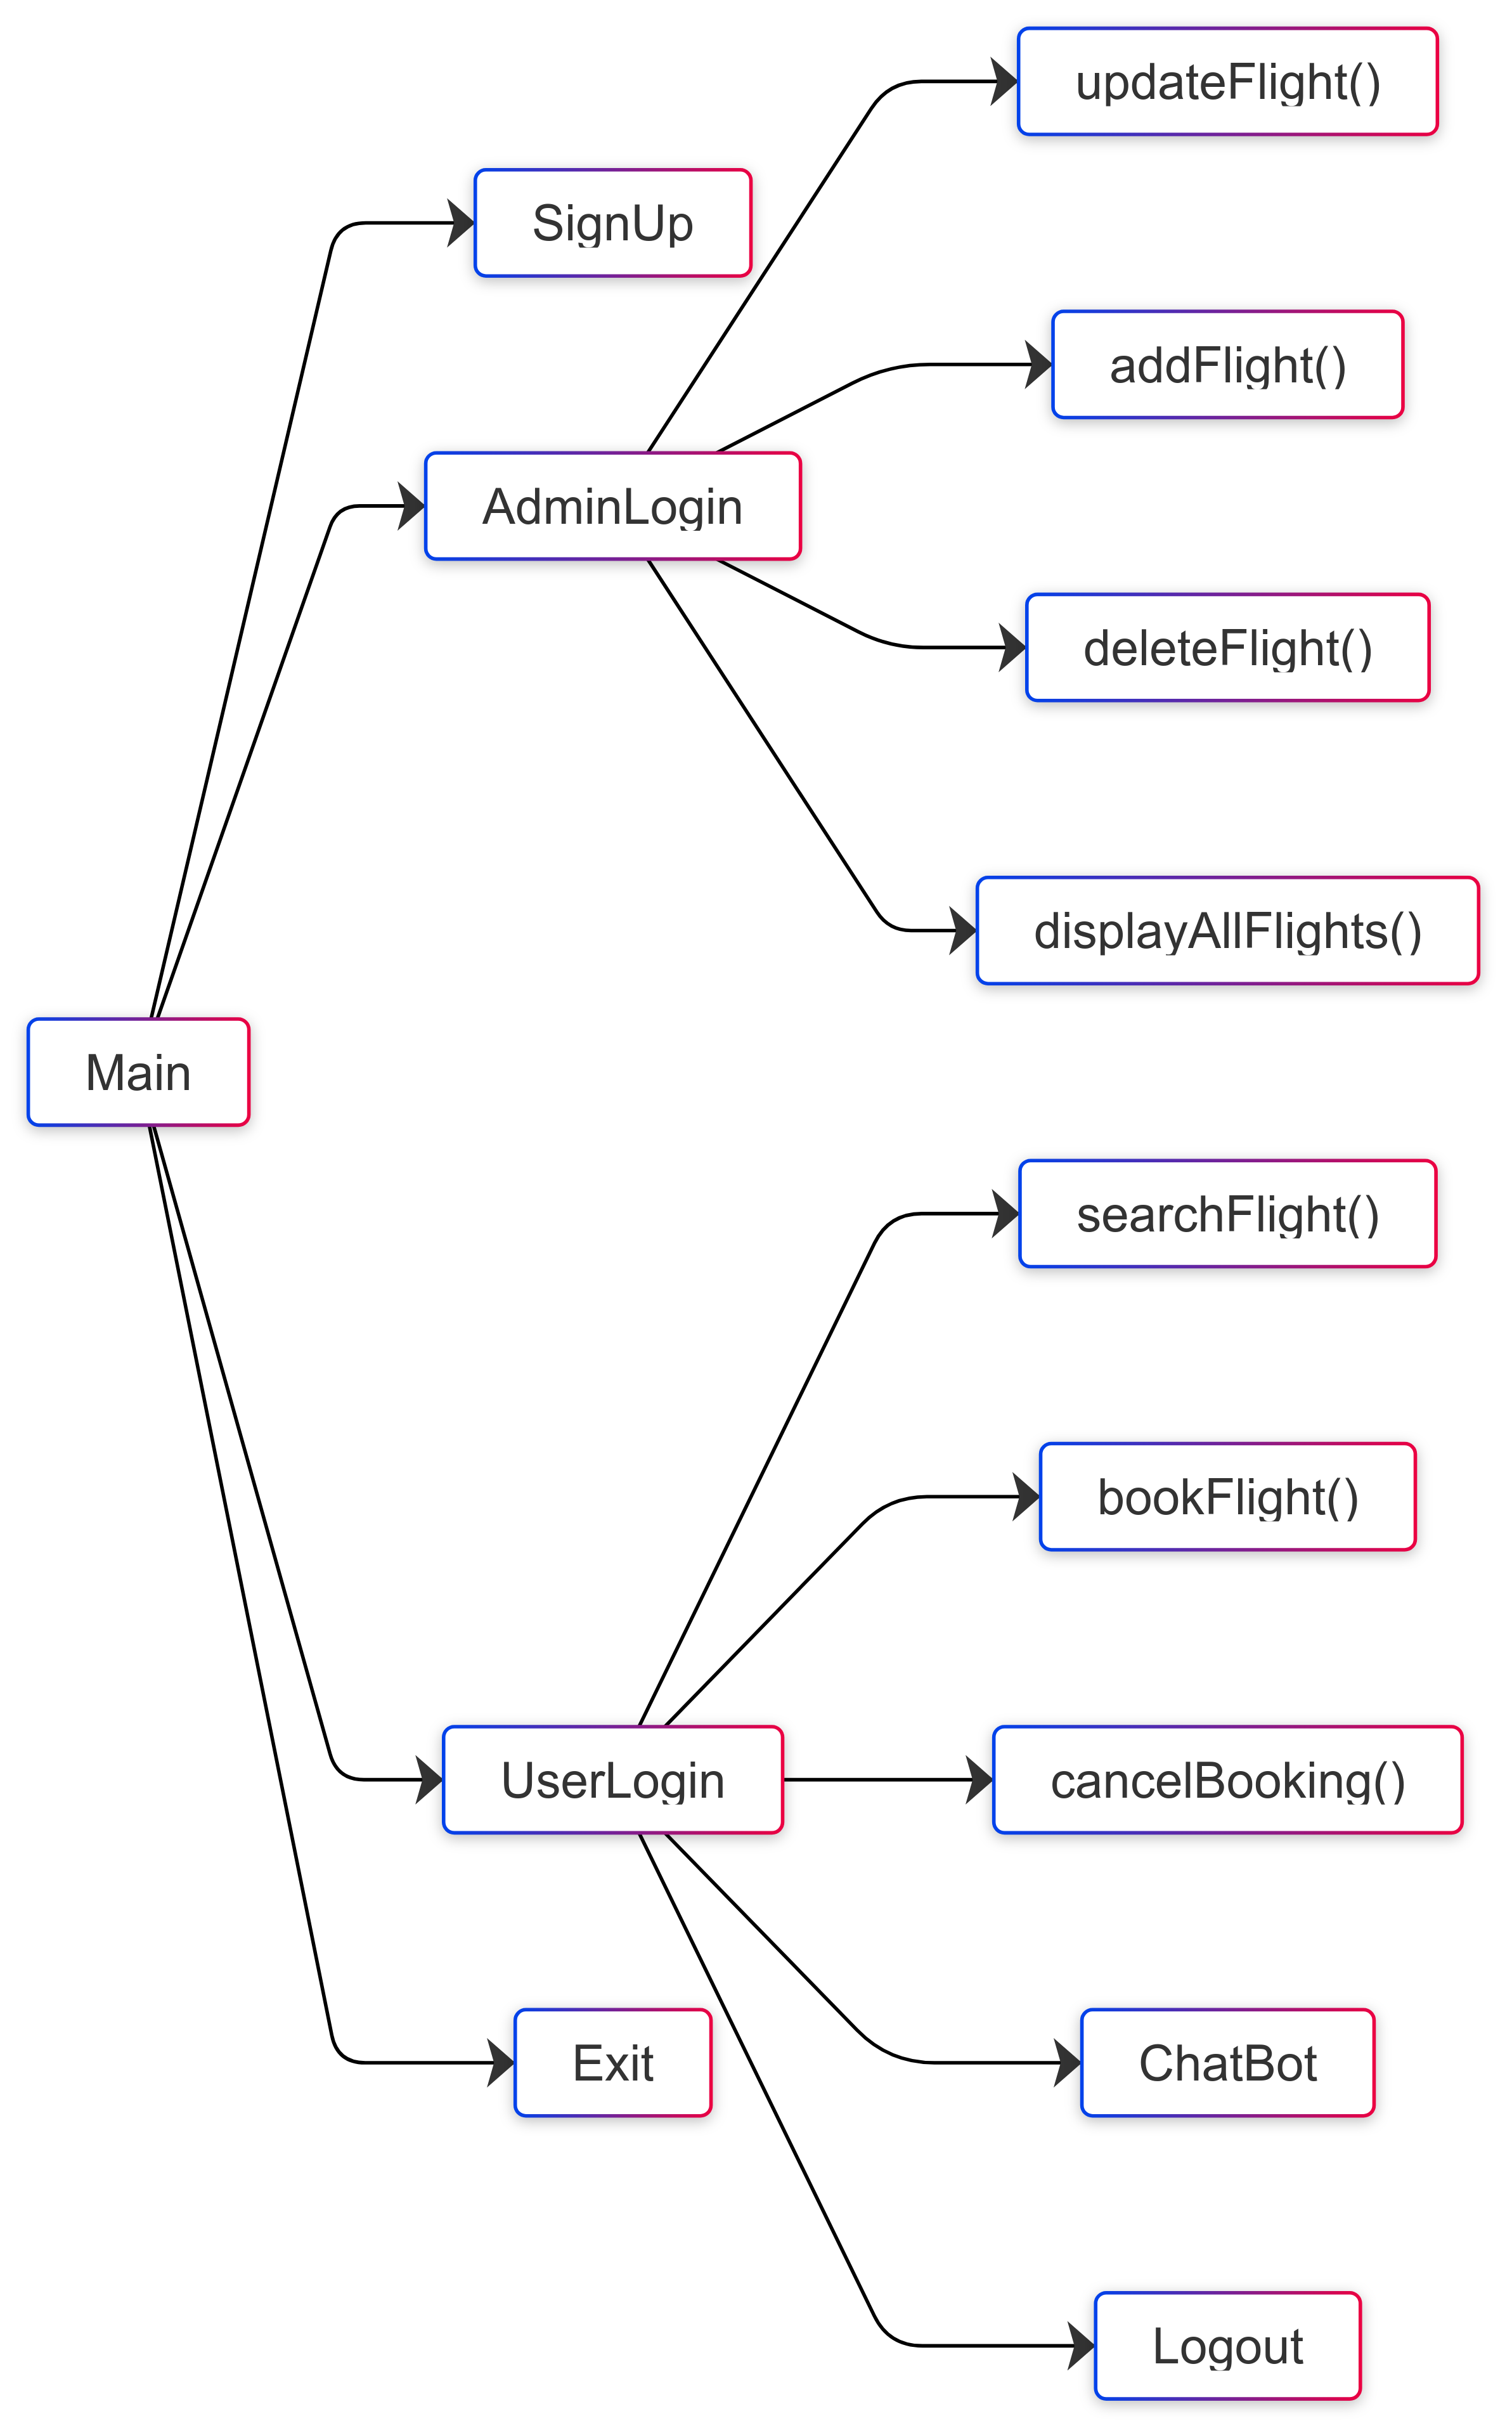
\includegraphics[scale=0.1]{main structure.png}
    \caption{Main structure of the Program}
\end{figure}


\section{Documentation}
\subsection{Functions for User Utilities}
The main Functions used in the User Utilities are as follows:
\begin{itemize}
    \item  \texttt{int searchFlight()}: This function is used to search for flights according to the source, destination, date. The function then searches for the flights according to the user's input and displays the flights available.\\
    \item \texttt{int bookFlight(char* flightnum, char* usr)}: This function is used to book a flight. The user is asked to enter the flight number and the number of seats to be booked. The function then books the flight and updates the booking history.\\
    \item \texttt{int cancelBooking(char* tick)}: This function is used to cancel a booking. The user is asked to enter the booking ID and the function then cancels the booking.\\
    \item \texttt{void view\_booking\_history()}: This function is used to view the booking history. The function displays the booking history of the user.\\
\end{itemize}
\subsection{Functions for Admin Utilities}
The main Functions used in the Admin Utilities are as follows:
\begin{itemize}
    \item \texttt{void addFlight()}: This function is used to add a flight. The admin is asked to enter the flight details and the function then adds the flight to the database.\\
    \item \texttt{void updateFlight()}: This function is used to update the details of a flight. The admin is asked to enter the flight number and the function then updates the details of the flight.\\
    \item \texttt{void deleteFlight()}: This function is used to delete a flight. The admin is asked to enter the flight number and the function then deletes the flight from the database.\\
    \item \texttt{void displayAllFlights()}: This function is used to display all the flights available. The function displays all the flights available in the database.\\
\end{itemize}
\subsection{Functions for Bandhu--the chatbot}
\section{Contributions}
\end{document}